\chapter{Implementation}
\label{implementation}

In this chapter, we will describe the most important classes of Metadata Extractor and explain their main responsibilities. The software consists of the main three parts which will be discussed - ER/Studio module, PowerDesigner component and Modeling Common, which is the shared part. 
The common module is a general artifact that is designed to be helpful when designing a metadata extracting tool from an arbitrary modeling tool and the tool is aimed to be integrated into the ecosystem of Manta Flow. \\

We go through classes and methods from the source code of Metadata Extractor from a higher perspective. 
Even though not every class, interface, and method are described in the chapter, a detailed programmer's documentation containing this information is attached in the form of JavaDoc.

\section{ER/Studio}

Now let us introduce the parts of Metadata Extractor implementation that are coping with data models product of ER/Studio Data Architect.

\subsection{File Reverse-Engineering Tool}
\label{subsec:dm1_tool}

In \Cref{subsec:dm1_format} we introduced the .DM1 file format, which is used for storing ER/Studio's outputs.
The file format consists of CSV tables and its inner organization of data resembles a relational database.
We need to decrypt the relations between the tables in .DM1 files, to be able to reconstruct objects stored in the files. That is because it is not easy to see, how structured information is stored in tables of the file format.
Relationships in this type of tabular data storage are realized via primary and foreign keys.
The task is to find out what tables are linked in the format, since it may uncover how complex objects are reconstructed to many interrelated tables.
For this purpose, we developed a little reverse-engineering (RE) tool which should help us to gain the knowledge necessary for reconstruction needed information from the files. \\

Input for the reverse-engineering tool is an arbitrary .DM1 file, while output must describe the logical layout of the file structure.
We observed the analogy of the file format's storage logic with relational databases. 
These databases can be represented understandably by a diagram.
Thus, it would be nice, if the output of our utility would be such a diagram capturing the organization of .DM1 files.
However, creating a relational diagram directly from the reverse-engineering tool would be too complicated. We may recall that for creation of relational diagrams modeling tools are used. The best solution would be to reuse this capability of theirs.
Modeling tools usually have the ability to transform selected routines of SQL into a visual representation.
For example, based on the statement "CREATE TABLE T" a modeling tool can draw a box in a diagram representing table T. 
By means of SQL, table columns and key constraints can be defined as well.
If there is a foreign key column in table B, which is at the same time a primary one in table A, it forms a relationship between the two tables, A and B. This relation is showed graphically in a diagram produced by modeling tools.

Therefore, if the RE tool is able to generate a SQL create procedure for each of the tables from ER/Studio's file format and to define primary and foreign keys on the tables afterwards, modeling tools can transform such code into a visual representation of the analyzed file format.

To define a SQL create statement for the tables of ER/Studio's file format is straightforward once a .DM1 file is parsed. For parsing, the tool uses the parser described in \Cref{subsec:dm1_parser}.

On the other hand, deciding which column of a table is primary, which columns are foreign keys and to what primary column every foreign key refers to, is a more complicated task.
We needed to take the reverse-engineering process one step further - to be able to infer keys from tables.
Modeling tools have the ability to obtain relationships between tables in a reverse-engineered relational database, however, the knowledge is based on metadata defining those keys. Databases can store such metadata, but plain SQL create statements that our RE tool produces, do not provide any additional information like that.
What we needed was a utility inferring relations between tables based solely on column names or/and content of database tables. However, we have not found any suitable already existing solution.
In this situation, we had no better option than to enrich our reverse-engineering tool of this ability.
The output of the RE utility, therefore, needs to be a SQL script containing definitions of tables, columns, and key constraints.

As the development of this utility is not the focal point of this work, the RE tool is not going to be an out-of-the-box general solution for deducing keys of relational databases and it is primarily concerned with the objects and properties picked by the analysis in \Cref{metadata_enumeration}. Even though, it should provide us the needed overview of .DM1 files organization.

We had to decide what programming language to use when creating the reverse-engineering utility. Although there may be scripting languages that would make some operations, like joins on tables, easier, we decided to use Java. Metadata Extractor itself is written in it and there is an important module - Parser that the column deducing utility and Extractor require. By developing both in Java it is possible to reuse the parser component. \\

Let us now describe the workflow of the RE tool.

To begin with, an analyzed .DM1 file is parsed into a set of instances of the class \classname{CsvTable}. When trying to find out what columns are key constrained, the idea is to look at the loaded tables from two different views.

The first perspective is to take into account only metadata of tables. 
This approach is represented by the class \classname{DependencyCreator}. 
It treats columns that look like keys (e.g., those which name ends with the "ID" suffix. The policies are determined by \methodname{isOnBlacklist} method) as if they were equivalent across all loaded tables.
The most important method in the class is \methodname{createDependencies}, which pairs potential key columns and tables containing the candidate columns.
Then the class \classname{RelationFinderByTableDefinitions} allows querying over the structure found by \classname{DependecyCreator}, showing what tables are possibly related through a series of joins.
Among others, there is a general method \methodname{getDependenciesWithPaths} showing the sequence of joins needed to do, in order to put together records from table A with those from table B.

The second view takes into account data stored in tables as well. 
When analyzing what are relations between tables, we consider a table being a collection of columns. The \classname{CsvColumn} class represents a column, storing its name and a set of values from all records of a single table at the position of the given column.
The \classname{RelationFinderByTableContents} class is used for this approach when further searching for key columns.
This way, the RE tool examines if columns with the same names have corresponding contents.

An instance of \classname{RelationFinderByTableContents} filters tables that have no content, thus are irrelevant for this approach.
The class has a method determining if a column can be considered the primary key of a table. 
That is true only if such a column contains solely distinct values, as a primary key must be completely unique in a table.
The relation finder also has a method finding out if a column can possibly be storing foreign keys. The idea is that if column A contains foreign keys referring to primary keys specified in column B, each entry of A must be present in B, thus A must be a subset of B.
What more, in .DM1 file format is a table \erstudiotable{Identity\textunderscore Value} that explicitly pairs tables with their primary key columns. 
The reverse-engineering tool takes advantage of this information as well.
The finder class also inspects if the primary keys are defined in some predefined order or if there is some similar pattern of how primary keys are listed in a .DM1 table.

The classes above allowed us to look from multiple perspectives at metadata and data of tables in the analyzed file format.
To put it all together, to finally generate the output in the form of SQL code defining .DM1 tables and their keys based on the analysis, the class \classname{TablesToSQLConverter} is used.
Its crucial method is \methodname{writeMySQLSource}. 
At the beginning it defines a SQL create statement for each table from an ER/Studio source file. 
Then takes place the phase of creating key constraints. 
It works with candidate columns that satisfy policies for key-containing columns defined in the \classname{DepedencyCreator} class.
Also, these columns must be present in at least one table, so one or more joins can be made using the keys the columns store.
The converter class also provides space for a manual definition of pairs table and its primary key that were identified by inspecting the file format using \classname{RelationFinder*} classes.
Then resolution of keys goes like this: at first place, primary keys defined by a user are set, then the information stored in \erstudiotable{Identity\textunderscore Value} table is used. Lastly, the key inference based on policies taking into account column names takes place. 
For example, if a column is called tableA\textunderscore id, it is very likely that it stores primary keys if it comes from a table called tableA.
If a column is set as primary key storage in one table, for each of the remaining tables that contain a column with the same name, the column is marked as a foreign key referring to the first table.
In the case that there are columns, which were chosen as candidates for being key containers, but no constraint was assigned to them in previous steps, it goes as follows. 
One table which contain the given column is marked as the source of primary keys and the remaining are considered to store references to the chosen table. The last approach may cause slight inaccuracies in the final result, but the main message should not get lost.

\subsection{Parser}
\label{subsec:dm1_parser}

We already discussed in \Cref{subsec:dm1_format} that the files storing objects we want to recreate from ER/Studio are using format, which is basically a sequence of CSV tables. 
In order to be able to further process the data saved in the file format, programs need to load the contents of those tables into corresponding data structures. That is what parsers are for.

Already existing CSV parsers are made to process a single CSV table per file. There is no unified definition for the comma-separated-value files, but usually, they do not allow naming CSV tables as present in .DM1 files.
What is important to say about a CSV table is that it consists of entries. 
Entry is located on a separate line and consists of fields and the last record is followed by a line break. 
Fields in an entry are separated by a comma.
A field may contain a comma or line break, then it must be enclosed in double quotes.
If a double quote appears in a field, it must be in the enclosed section and the quote itself must be doubled \cite{RfcCSV}.

What more, the structure we need to parse consists of many CSV tables. Each of them has its name, definition of columns (a special entry that is the first entry in a table and its fields are names of columns), and entries.
Two tables are separated by a single empty line.

Putting it all together, it seemed to be easier to develop our own parser for .DM1 files that processes the files into a set of tables identified by their names.

A single table is represented by an instance of the class \classname{CsvTable}, which contains its name as a string, references definition of its columns stored in a realization of the class \classname{CsvColumnDefinition}, and finally holds records themselves, they are instances of the \classname{CsvColumn} class.

However, the view on a table may vary by a specific usage of the parser. 
Using the reverse-engineering tool (\Cref{subsec:dm1_tool}), we inspected what values are stored in columns, examined ranges of values across all records of a table, etc.
On the other hand, if we see a table as records, where each record has properties, one property corresponding to one column, from this perspective a table is a set of rows.
The second case is required by Metadata Extractor when it is reading the contents of a table for the sake of obtaining saved records. 
Once the most important responsibility of parser is correct - recognizing individual parts of a CSV table, the module can be modified easily to produce data structures compliant with either of the views.

Getting the name of a table is an easy job, as the name is represented by a single line of text. 
To resolve a record - to get the individual fields separated by a comma correctly, is a slightly more challenging task since the rules described at the beginning of the chapter must be taken into account.
We designed an automaton that accepts well-formed records of a .DM1 CSV table and recognizes its fields.

We propose a non-deterministic finite automaton, even though it can be translated to a deterministic one, we consider the NFA to be more clear and descriptive in this situation.
Set of states is $Q = \left\{i, q, e, a, f\right\}$.
Alphabet $\Sigma$ is a set of chars that can appear in a string, since that is what the automaton processes, together with $\lambda$ - an empty string.
$i$ is the initial state.
Transitions are illustrated in the following Figure 5.1.

\begin{figure}[H]
	\begin{center}
		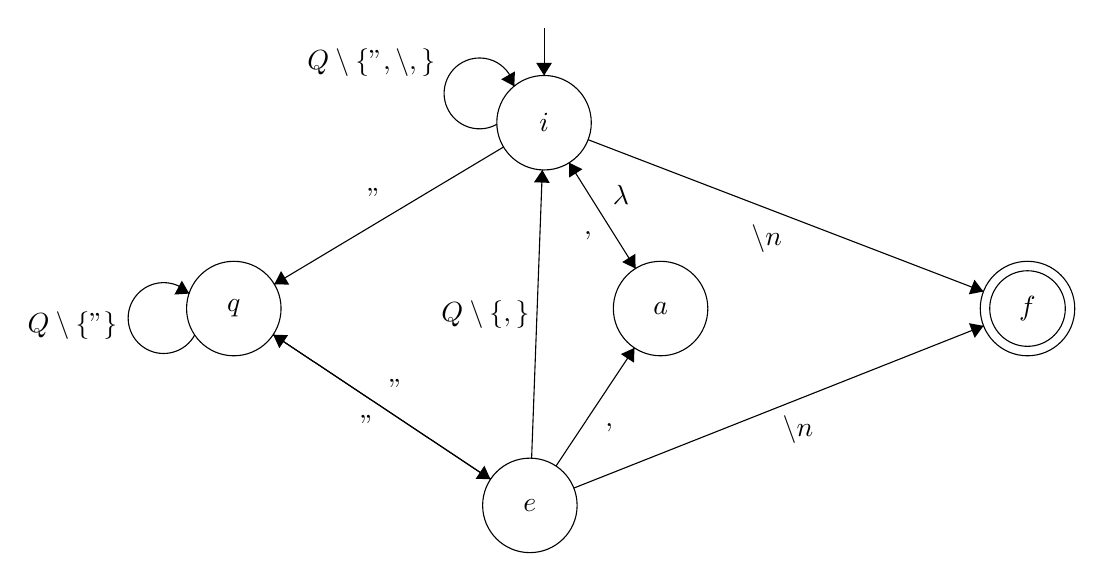
\begin{tikzpicture}[scale=0.2]
		\tikzstyle{every node}+=[inner sep=0pt]
		\draw [black] (40.8,-21.4) circle (3);
		\draw (40.8,-21.4) node {$i$};
		\draw [black] (71.5,-33.2) circle (3);
		\draw (71.5,-33.2) node {$f$};
		\draw [black] (71.5,-33.2) circle (2.4);
		\draw [black] (21.1,-33.2) circle (3);
		\draw (21.1,-33.2) node {$q$};
		\draw [black] (48.2,-33.2) circle (3);
		\draw (48.2,-33.2) node {$a$};
		\draw [black] (39.9,-45.7) circle (3);
		\draw (39.9,-45.7) node {$e$};
		\draw [black] (40.8,-15.4) -- (40.8,-18.4);
		\fill [black] (40.8,-18.4) -- (41.3,-17.6) -- (40.3,-17.6);
		\draw [black] (37.813,-21.495) arc (299.55605:11.55605:2.25);
		\fill [black] (38.91,-19.09) -- (38.95,-18.14) -- (38.08,-18.64);
		\draw (33.93,-17.59) node [left] {$Q\setminus\left\{",\backslash,\right\}$};
		\draw [black] (43.6,-22.48) -- (68.7,-32.12);
		\fill [black] (68.7,-32.12) -- (68.13,-31.37) -- (67.77,-32.3);
		\draw (54.94,-27.83) node [below] {$\backslash n$};
		\draw [black] (38.23,-22.94) -- (23.67,-31.66);
		\fill [black] (23.67,-31.66) -- (24.62,-31.68) -- (24.1,-30.82);
		\draw (30.04,-26.8) node [above] {$"$};
		\draw [black] (18.622,-34.87) arc (-28.28273:-316.28273:2.25);
		\fill [black] (18.27,-32.25) -- (17.8,-31.43) -- (17.33,-32.31);
		\draw (13.73,-34.26) node [left] {$Q\setminus\left\{"\right\}$};
		\draw (39.91,-33.56) node [left] {$Q\setminus\left\{,\right\}$};
		\draw [black] (23.6,-34.86) -- (37.4,-44.04);
		\fill [black] (37.4,-44.04) -- (37.01,-43.18) -- (36.46,-44.01);
		\draw (29.59,-39.95) node [below] {$"$};
		\draw [black] (42.69,-44.6) -- (68.71,-34.3);
		\fill [black] (68.71,-34.3) -- (67.78,-34.13) -- (68.15,-35.06);
		\draw (56.92,-39.97) node [below] {$\backslash n$};
		\draw [black] (41.56,-43.2) -- (46.54,-35.7);
		\fill [black] (46.54,-35.7) -- (45.68,-36.09) -- (46.51,-36.64);
		\draw (44.66,-40.78) node [right] {$,$};
		\draw [black] (37.4,-44.04) -- (23.6,-34.86);
		\fill [black] (23.6,-34.86) -- (23.99,-35.72) -- (24.54,-34.89);
		\draw (31.41,-38.95) node [above] {$"$};
		\draw [black] (40.01,-42.7) -- (40.69,-24.4);
		\fill [black] (40.69,-24.4) -- (40.16,-25.18) -- (41.16,-25.22);
		\draw [black] (46.61,-30.66) -- (42.39,-23.94);
		\fill [black] (42.39,-23.94) -- (42.4,-24.88) -- (43.24,-24.35);
		\fill [black] (46.61,-30.66) -- (46.6,-29.72) -- (45.76,-30.25);
		\draw (45.13,-26.01) node [right] {$\lambda$};
		\draw (43.87,-28.59) node [left] {$,$};
		\end{tikzpicture}
	\end{center}
	\caption[NFA Accepting a CSV Line]{Non deterministic finite automaton accepting a record of a CSV table in .DM1 file. In the state $a$ and $f$, the end of a CSV field is recognized and added to the record.}
\end{figure}

When loading a CSV record consisting of multiple fields not only the parser must determine the end of an entry, but has to collect its fields correctly as well. That is what the, at first sight redundant, state $a$ expresses. Once the automaton gets to the state $a$, the end of a field in the input is indicated. 
The boundary of the last field of an entry is, however, recognized in the accepting state $f$.

The parser's interface is a single method - \methodname{readFile}. It takes a file to process and returns table name and instance of \classname{CsvTable} pairs.

\subsection{Model}

The purpose of the Model component is to provide read access to both a raw structure of a processed source file and a fully loaded hierarchy of objects Metadata Extractor has reconstructed from a file.

The crucial objects and the important properties of theirs which Model is required to capture result from the analysis of ER/Studio data models listed in \Cref{metadata_enumeration}. They are described by functionality that is expected from them, making Model a set of interfaces. Here we describe them in more detail.

The perspective of a raw file structure loaded to memory is represented by the interface \classname{ErStudioFile}, where either all tables from a file can be retrieved via \methodname{getAllCsvTables} method or a single table may be obtained by its name using the \methodname{getCsvTable} method.

An ER/Studio solution - a set containing one logical data model and an arbitrary number of physical models, implements the \classname{ErStudioSolution} interface. All the objects contained in the data models of a solution can be retrieved using the interface's methods. A solution is defined in a file, the relative name of the file where the solution is an internal one is returned when called \methodname{getFileName}.

A .DM1 file is not restricted to store solely objects from a single solution but may reference external models (objects that are originating in another solution) as well, thus there can be objects from multiple solutions saved in a file. Each object is assigned to a solution where it originates.
If the name of the object's origin solution is identical with the name of .DM1 file from which it was loaded, it is an internal object, otherwise, we call it external. There is a single internal solution per .DM1 file. 
The overall structure of a file is represented by a realization of the \classname{ErStudioFileModel} interface that consists of a single internal solution and the file may reference some external solutions.

A base behavior of both logical and physical data models is defined in the \classname{DataModel} interface.
A data model has a name and contains owners. An instance fulfilling \classname{DataModel} contract must have property of type \classname{AbstractionLayer} set to either \methodname{Logical} or \methodname{Physical} just like every underlying object in a model.
It must be invariant that the whole subtree of objects, a root is a data model, has defined the same abstraction layer.

\classname{PhysicalDataModel} interface requires an additional feature - its realization can tell the database platform it is designed for. 
In the enum class \classname{Platform}, all the database management systems ER/Studio supports are captured with an extra entry for an unknown DBMS.

Models are storing instances of complying with the \classname{Owner} interface. An owner is either logical or physical according to what objects it can own and what type of model it may belong to. 
It has a name and allows access to the objects owned.

The generic interface \classname{Mappable<T>} is used by objects that can be mapped to \classname{DataObject}s (see the following paragraph) which are on the different abstraction level. The type parameter defines what is the specific kind of the mapped counterpart.

Important objects in a data model that can be described further by definition and note, while having a name extend the general \classname{DataObject} interface which extends the general \classname{NodeMetadata} contract (see \Cref{modeling_common}). 
These can be either \classname{CompositeDataObject} or \classname{SimpleDataObject}.

An interface for composite objects describes what features are expected from a table or an entity.
The two types have the very same set of properties that is why a single class is enough to capture both. 
Which of the two kinds an instance represents is decided by its \classname{AbstractionLayer} attribute - the logical layer indicates an entity, the physical a table.
A composite one can be mapped to another \classname{CompositeDataObject} and may contain simple objects.

The \classname{SimpleDataObject} interface is used to represent columns or attributes. Equivalently, the layer of abstraction is crucial to determine, whether an object fulfilling a simple object's contract can be stored in \classname{PhysicalDataModel} or \classname{LogicalDataModel}.

The reason to represent the pairs of, at first sight, different concepts of tables-entities just like columns-attributes in a single class is based on how ER/Studio treats them internally. Given that columns and attributes, tables and entities equivalently, are stored in a single CSV table and the distinction whether an object is of one or the other type is made based only on the fact to which data model, physical or logical, it belongs to.
The two types have the very same set of possible attributes. 
Even data models are treated similarly, only there is the additional attribute related to DBMS type in the case of physical models, while the logical ones do not need such information.

\subsection{Resolver}

The Resolver unit is here to provide the construction logic for building the objects which the model component describes.

Outline of what the Resolver module does is that using an instance of the \classname{ErStudioFileModelBuilder} class it creates the whole structure representing an input .DM1 file as an object described by the \classname{ErStudioFileModel} interface. 
It builds an internal solution, puts inner objects to maps-to relation, then loads external objects and at the end resolves mappings that lead across solutions using an instance of the \classname{ExternalMapper} class.
Parser provides an input for Resolver.

Typically, for each Model's interface we create an implementation. 
In Java, it is usual to call the classes fulfilling a contract \classname{*Impl} where * is a placeholder for the name of an interface. We stick to this naming convention. 
The \classname{*Impl} classes, in contrast to the interfaces that are used to describe Model, need to dispose of methods for setting up and adding properties or sub-objects. These classes can be found in the "imp" package. \\

We defined what is expected from the objects collected by Metadata Extractor and added the functionality to set up these objects.
So the last missing piece of the puzzle needed is to put together the gathered information to recompose the final objects and their metadata.

The logic taking care of the objects reconstruction can be found in the Resolver's package "build".
The skeleton of how an instance of \classname{ErStudioSolution} is created is prescribed by the method \methodname{buildErStudioModel} in the class \classname{AbstractDataObjectsBuilder}. The method follows the paradigm of the template method design pattern and defines the steps needed to take, in order to construct an instance of \classname{ErStudioSolution} solution, no matter if it is of the internal or external type.
The template enforces a tree of objects in a solution that is built from the top to the bottom.
The very first step is to create a root of such tree - an instance of \classname{ErStudioSolution} that is being built, then \classname{DataModel} structures from the solution are loaded, underlying \classname{Owner} implementations follow, \classname{CompositeObject} realizations after, and finally \classname{SimpleObject} instances. 
Child objects are attached to their parents just after they are created.
The abstract builder contains common methods for the construction of the needed objects. 
Those methods are not dependent on representation, they only require a set of properties as the input, to build the resulting objects from. 
The groups of properties needed to be collected about each type of complex object from a data model to proceed the construction are described by the interfaces in the package " modeledobjectproperties".

The specific way of gathering information about objects to be reconstructed is tied with details of how the objects are saved. 
Concrete builders realized by the classes \classname{InternalDataObjectsBuilder} and \classname{ExternalDataObjectsBuilder} provide implementation of the abstract object builder.
In the case of an internal solution, information about objects is retrieved from CSV tables, where for each table there is a dedicated and references across the tables are resolved.
On the other hand, in the case of external solutions, they are fully represented in a single CSV table that stores XML structures describing these objects. 
\classname{ExternalDataObjectsBuilder} uses a simple SAX XML parser to retrieve the data required for object reconstruction from the XMLs.

\classname{InternalDataObjectsBuilder} has one more responsibility, it is to create mappings between \classname{Mappable} objects in the internal solution with a help of \classname{InternalMapper}. 

The \classname{InternalMapper} class only has knowledge about the layout of a CSV table containing internal mappings. Similarly, the \classname{ExternalMapper} class knows about the layout of the table storing external mappings.
However, the logic of putting objects to maps-to relation is coded in their common predecessor of these two classes - \classname{AbstractMapper}.
The mapping logic goes through a given CSV table, which definition fulfills the interface \classname{MappingTable} and links pairs listed in the table by mapping, if the objects to be mapped are compliant.

\subsection{Reader}

The Reader component puts together Parser with Resolver and produces data structures described by the model component. \\

An instance of the \classname{ErStudioDm1Reader} class crawls through a directory with input .DM1 files and processes them. 
Each time the \methodname{read} method is called, it forwards the next file from the input folder to the parser. Result of the parser is handed to Resolver, which produces a result fulfilling the contract of \classname{ErStudioFileModel} and that is what the \methodname{read} methods returns.

\subsection{Data Flow Generator}

Having constructed the objects defined in the model unit, Metadata Extractor sends them to the Data Flow Generator unit, where an instance of \classname{ErStudioSolution} gets transformed into an output graph. This component puts together the functionality of Manta Flow with Metadata Extractor.

Before describing the workflow of the generator unit, let us mention its layout.
There is a scenario that executes independent tasks. A task is a routine that has an input and an output. In our case we use a single task, whose input is a data structure described by the model unit and output a graph with extracted information.

Namely, realization of the class \classname{ErStudioDataflowScenario} reads an input file, and executes the task - given by an instance of the \classname{ErStudioDataflowTask} class. 

The method which tasks must override and gets called is the \methodname{doExecute}. In this particular task it is needed to go through the whole hierarchy of the input data structure - \classname{ErStudioFileModel} unroll solutions - internal as well as external.

It is crucial to identify what database an extracted physical data model corresponds to.
This is important for Metadata Extractor to be able to pair physical data model objects with those from database dictionaries. The correct pairings allow Manta to interpolate technical lineage on the logical layer, as well it brings extracted metadata to database objects in the technical lineage.
A suitable realization of the \classname{Connection} class corresponding to a physical data model is made of information extracted from a data model - DBMS type and schema, the remaining details - database name, server entered by a user in a .ini file.

Once the connections are assigned to physical models, Metadata Extractor traverses trees of data models, and creates nodes using a realization of the \classname{DatabaseConnector} interface in the case of physical level. 
When it comes to logical objects, Metadata Extractor takes an advantage of an implementation of the \classname{DataModelNodeCreator} interface (both contracts and their default realizations are defined in the modeling common component described later \Cref{modeling_common}).

The only item left is to create mapping edges for the corresponding nodes.
Metadata Extractor creates the mappings symmetrically when resolving. It means the full information is captured on both interconnected levels. 
This way, it is possible to create all the mapping edges by going through all objects from a single level of abstraction, no matter which level as each mapping edge is contained in both of the levels.
Thus, Data Flow Generator goes through all the logical objects, creating their node representation and collects the attributes that have to be linked to a column.
When a node representation of physical objects is takes place Metadata Extractor checks if the just constructed node has a mapping, a MAPS\textunderscore TO edge is set between the logical and physical node.

\section{PowerDesigner}

Now we move on to describe the implementation of Metadata Extractor's components which process data models created by SAP PowerDesigner.

\subsection{Parser}

To load data models that are the output of PowerDesigner and to reconstruct objects they save, Metadata Extractor needs to parse them. The files are of XML type.
In the analysis section, we already discussed the possibilities when it comes to reading XML files. We concluded that the most suitable approach for us should be loading inputs to a DOM tree data structure.
We did not try to reinvent the wheel, as there are many DOM parsing services that can be reused. 
Given that in the ecosystem of Manta software there is present an internal artifact capable of transforming XML to DOM, Metadata Extractor will make use of it.

\subsection{Model}

The Model component is the mean we use for the description of the main modeled objects that Metadata Extractor has to obtain
Let us start describing these objects generally.

Thus the \classname{DataModel} interface requires the name of the file where it is stored and its children.
Then the hierarchy of objects goes like this: a model has at least one realization of the \classname{Schema} interface, schemas store instances of the \classname{CompositeObject} interface, which contains implementations of the \classname{SimpleObject} contract.
Every PowerDesigner's data model is stored in a separate file, thus a data model is identified uniquely by where it is stored on disk.
This basic tree structured skeleton is present in each of the three data models - conceptual, physical and logical. 
What more, on the logical and conceptual level, since they are represented by an EER diagram, an entity can inherit from another one, thus the interface \classname{Entity}, which introduces the concept of a parent entity, will be used by on these layers. 
Each of the important objects may have some metadata providing further description and extends the interface of \classname{NamedObject} (see \Cref{modeling_common}).
These interfaces are generic and provide a common basis for corresponding specific interfaces.
For every model type, there exists a package, where those specific contracts of modeled objects lie. 
The concrete interfaces, on one hand, take over the common concepts, while on the other hand may be easily extended, once a new functionality, which is specific for any abstraction level, is identified.

\classname{Mappable} interface is present to capture objects that are in maps-to relation. It realized via instances of \classname{CompositeObject} or \classname{SimpleObject}, however a target of a mapping is a string every time - it is a globally unique ID of the mapped counterpart, not another instance directly. That is because mappings in PowerDesigner leads across different files, thus an actual representation of the counterpart may be unreachable yet.

\subsection{Resolver}

The Resolver component provides means of creating objects, which are described in Model using data that DOM parser obtained from an input file. The output of Resolver is an instance of \classname{DataModel}.

Abstract classes, prefixed with \classname{Abstract*}, capturing common concepts are present to minimize code redundancy and to provide a unified way to handle similar objects, even though they do not represent any complete object of a data model. 
The actual objects that have backing in data models are implemented via \classname{*Impl} classes.

The construction logic of a data model is concentrated in the "build" package.

The API for creating a data structure representing a data model is simply defined by the  \classname{DataModelBuilder} class, which is containing the method \methodname{buildDataModel}. And once a model is built, the result can be collected from \methodname{getResult} operation.

Despite the API for data model creation is unified, there is a different strategy used for building each of the data models, based on abstraction level. 
Therefore, when processing a PowerDesigner file Metadata Extractor must choose the suitable implementation of \classname{DataModelBuilder} accordingly. 
The class \classname{BuilderFactory} is used to choose the correct builder via its factory method which implementation - \classname{PhysicalDataModelBuilder} or \classname{LogicalDataModelBuilder} or \classname{ConceptualDataModelBuilder} by the abstraction level of the data model file that is about to be resolved.

The outline of how the builders work is proposed in their common base class \classname{AbstractDataModelBuilder}. 
Also, the functionality independent of the type of a specific data model is written here, the way to do it is to look on objects from the perspective of abstract classes that are providing the general features needed for the process of data model creation.

The specific implementations take advantage of the fact that forming a tree-like structure from an XML format is natural and straightforward. That is why, for now, Metadata Extractor omits a general view on the construction of a data model. Ignoring the convenient structure of the XML tree would hide the context provided straightforwardly by DOM nodes. 
Requests for specific DOM nodes during the process of object creation are done using XPath queries on the fully loaded XML document.

\subsection{Reader}

The Reader component interconnects Resolver and Parser. Input for this component is a directory, where the reader searches for files containing saved data models. It collects a batch of files from the input directory, loads them using the two components, and sends the batch in the processed form of a set of \classname{DataModel}s to the Data Flow Generator unit.

Input directory containing PowerDesigner files to process is the input for the reader's most important class \classname{PowerDesignerXmlComponentReader}. 
The reader recursively discovers the directory and collects the file that will have to be resolved using the \methodname{collectFiles} method. 
When a data model file is found, its dependencies are checked using a \classname{SAXParser} with a simple handler class \classname{TargetSAXHandler}, which is obtaining paths to related models from an XML.
The found dependent files, however, must be in the input directory, so if it is not the case, the reader tries to resolve their paths and check if there is no file with matching sub-path within the input directory. If it is a bidirectional edge between the files is created. 
Once all the files from the input are collected, component creation takes place so the input set is split into smaller logically connected groups.

When the main API method of Reader - \methodname{read} is called, Parser and Resolver start processing one component. Result of their work is a set of related reconstructed \classname{DataModel}s which is the return value from the method. 
That means the reading method is stateful and \methodname{canRead} checks if there are any component left to be returned.

\subsection{Data Flow Generator}

The purpose of this component is to create a correct graph representation for the objects described in the model component. Data Flow Generator has to collect information to identify databases that physical models resemble.

When translating a set of reconstructed data models and their underlying objects, a suitable instance compliant with the \classname{GraphBuilder} interface must be chosen based on the level of abstraction for each data model in the input. Metadata Extractor does it using the \classname{GraphBuilderFactory} class.
Then the tree of data model objects is traversed.

When dealing with a physical data model, an instance of \classname{PhysicalGraphBuilder} is used, underlying \classname{DatabaseConnector} searches for the modeled database objects. 
A suitable \classname{Connection} realization corresponding to a physical data model is made of the information from a data model and .ini file, as loading connection details from .dsn and .dcp files is not supported yet. A user has to specify in the .ini file type, server and name of a database for a physical data model, in order to identify the corresponding database successfully.

On the other hand, physical and logical data models use the generic \classname{ModeledGraphBuilder} class for creating nodes representing objects obtained from data models of higher abstraction.

Lastly, during the phases of translation objects to nodes, Metadata Extractor collects by IDs the nodes that have a mapped counterpart.
Once all the data models in the processed components are fully built, the generator can resolve the mapping, as both ends of the MAPS\textunderscore TO edge must be present. 
Then Metadata Extractor simply looks at to what ids are objects mapped, obtain an actual representation of these ids put them into the relationship by creating the edge.

\section{Extensibility - Modeling Common}
\label{modeling_common}

For the sake of general information retrieval from modeling tools, we developed a unit where a component for metadata extraction from an arbitrary modeling tool meets Manta Flow.
This module, where the common bridging logic is stored, we call Modeling Common.

Physical data models need to be paired with corresponding connections to DBMS in order to identify the database they resemble. 
Only with this knowledge, Metadata Extractor can correctly pair the same database objects that appear both in a physical model and in a database dictionary extracted by Manta Flow from a live database. 
This functionality is provided by implementations of the interface \classname{DatabaseConnector}. Details about the target database of a physical data model are kept in a realization of the \classname{Connection} contract.
The API to database dictionaries created by Manta is provided by the \classname{DataflowQueryService} interface. 
Having collected information of a physical object, either a column or a table, the query service tries to find the object in the dictionaries using \methodname{createColumnNode} or \methodname{createTableNode}. 
If the service succeeds, matched node from a dictionary is appended to the output graph, otherwise null is returned from a \methodname{create*} method and Metadata Extractor tool copes with the situation in such a way that it constructs a node that has no backing in a live database, marking the node's attribute source type to MODEL to make clear in the output, that it is an artificial node based only on a physical data model. 
It can be from two reasons - the database object does not exist or we provided inaccurate/incomplete data to identify it.

So the first requirement for a general extractor from data modeling tools is to be able to organize extracted metadata in such a way that \classname{DatabaseConnector} may be called and ideally matches the modeled objects with the extracted ones.
This is a very important step, as this pairing is the prerequisite for business data lineage creation. If the physical modeled objects do not match the ones from a database that take part in data lineage, there is no flow to be propagated to higher levels of abstraction via MAPS\textunderscore TO edges and the result of interpolation will be an empty set of edges.

Secondly, we have defined a common way of creating nodes representing objects extracted from data models of higher abstraction than the physical ones - conceptual and logical.
We define a set of methods, where each of them is responsible for the creation of node representation of a type of object that may appear in the data models. Most commonly, a modeling tool will support only a subset of the object types the node creator is able to construct. 
However, that is not a problem as the node hierarchy is not that strict and it can be built to be compliant with the layout of a specific modeling tool. 
For example, it is not necessary to build an attribute under an entity node if a modeling tool does not allow such a concept, just like an owner node is not necessary, as there is no strict rule if the tools should support it or not.

We have discussed the modeled objects on the conceptual and logical level are described by ER or EER diagrams. 
The important fact is that the possible kinds of objects are going to be very similar in both models, that is why the single interface \classname{DataModelNodeCreator} for high-level node creation may be used.
However, it must be implemented by two different classes \classname{LogicalDataModelNodeCreatorImpl} and \classname{ConceptualDataModelNodeCreatorImpl}, so details about node's type can be specified, therefore the nodes will not mix between the layers.
A realization of the \classname{Resource} interface differentiates technologies, in our case it makes sure objects extracted from modeling tools are aggregated by what specific tool is their origin.

To draw an object as a node and attach its metadata to a node, such as definition or comment, the \classname{NodeMetadata} interface should be implemented by the object that is being transformed into a node representation.
The contract forces the implementers to define a name for the node and to expose the metadata to be attached to the node representing them in the output in the form of strings. 
More precisely, the objects have to override the \methodname{getName} method and to fill a \classname{Map<String, String>} data structure where a key is the name of a property. 
The metadata accessible in the map are shown when presenting the output graph and further describes the extracted objects. \\ 

To create a guideline what to do when implementing a metadata extraction from a different modeling tool is the following:

\begin{enumerate}
	\item Define the crucial data model objects, relations between them, hierarchy and properties interesting enough to be captured in data lineage by read-only interfaces. That is the model component. 
	The objects that will be represented as standalone nodes in data lineage visualization at the end have to implement the \classname{NodeMetadata} interface.
	\item Depending where from the data models are obtained, this phase generally retrieves data models from storage. It may be by calling a web API to get data mode objects from a server, retrieving them from a database, or like in the case of Metadata Extractor, by parsing a file.
	\item Resolving takes place once a representation of data models was obtained. This stage transforms the acquired structures into objects conforming the aspects described by the model module.
	\item Data flow is generated from the output of Resolver. This module translates data structures describing modeled objects to graph nodes. 
	Database objects from physical data models are expected to match the ones in database dictionaries of Manta that were extracted directly from databases. 
	The communication with Manta is done via \classname{DatabaseConnector} interface and a concrete \classname{Connection} that is assigned to a physical model.
	Logical and physical modeled objects are transformed to node representation using the corresponding implementation of the \classname{DataModelNodeCreator} interface - logical and physical respectively.
	Once the nodes are created out of the extracted objects, the resolving of mappings between the layers takes place.
	Linking correctly physical nodes that were paired with the ones from the database dictionary, with higher level nodes is crucial to bring business lineage. 
	However, there is no strict skeleton for this process as the approaches to how modeling tool realizes mapping across data models may be substantially different, as we have seen in case of PowerDesigner and ER/Studio.
\end{enumerate} 

\section{Error Handling}

We require Metadata Extractor to be as stable and as robust as possible. 
When an unexpected event occurs, the program should not fail on an exception and stop computing. Metadata Extractor should ideally print a message describing the given event to log using the SLF4J logger with level \methodname{error} or \methodname{warn} depending on the severity. 

If there is something wrong in a data model definition, Metadata Extractor tries to get as much information as possible.
For example, if a part of an XML tree describing one PowerDesigner table is malformed, partial information about the table should be extracted so the program tries to retrieve it. In case the table is damaged irrecoverably, it should be skipped and continue with the processing of other tables directly. 
One way or another, one wrong table must not affect any other table in the given file.

\section{Technologies}

The quality of the programmer's toolbox may have a huge influence on his productivity when developing a more complex piece of software.

\begin{itemize}
	\item Java 8 \\
	To be able to integrate Metadata Extractor into the ecosystem of Manta Flow the best solution is to use Java as the APIs of the data lineage software are written in this programming language.
	\item Maven \\ 
	For dependency management, the most usual tool when programming in Java is used - Maven. In order to build the program, all the Manta Flow artifacts which Metadata Extractor depends on must be obtained successfully. However, those artifacts are reachable only within Manta's private network.
	\item Spring \\
	For program configuration, inversion of control via Spring's XML files is used. Along with .properties, where variables used in the spring files may be (re)defined.
	\item JUnit 4 \\ 
	The standard for unit testing Java programs is the JUnit framework we use.
\end{itemize}

\section{Testing}

Automated unit tests validating the crucial parts of the implementation makes much easier to determine the correctness of Metadata Extractor's logic. 
We developed test suites that should tell in what shape is the program.

\subsubsection{ER/Studio Parser}

The correctness of the parsing process is checked by the class \classname{ErStudioFileFormatParserTest}, which is controlling how many CSV tables from a parsed .DM1 files were obtained. Given that the format consists of a constant number of tables if the count is mismatching it indicates a flaw in detecting borders of tables.
Also, every CSVs should be valid in the way that each row in a table must have the same number of fields. If it has not, we assume there is a problem on our side and parser does not pass the tests.

\subsubsection{Reader \& Resolver}

The testing output of the Reader module shows a lot about Resolver's correctness since the logic of the reader is actually provided by this module. 
By the nature of Reader - it connects Resolver and Parser, these tests rely on the fact that parser works correctly and we assume this is true as far as the parser module tests are passing.
The goal of Reader tests is to find out whether all objects from input data models were successfully and correctly loaded into data structures described by the model component.
In the case of ER/Studio, the testing compares expected statistics about data models such as the number of physical models in a solution, entity count of the logical model, etc. with the number of objects that were loaded actually by the reader.
Secondly, some specific objects from the hierarchy of a data model that is on input are picked and checked if they were loaded accordingly. Tests check metadata of those objects and mappings with other objects as well. \\ 

PowerDesigner must create components correctly, so we have a test for checking if the number of components is correct and if dependencies on files with obsolete path can be fixed.
The main Reader test consists of reading file by file, thus the size of a component is one every time (the components creation correctness is ensured the previous test).
The expected values and objects are loaded from JSON sources file where they are stored in a deserialized form.

\subsubsection{Data Flow Generator}

In Data Flow Generator module, we are interested if objects loaded by Reader are transformed into nodes as expected.
The skeleton is similar for both modeling tools. \\

\classname{*GraphBuilderTest} classes are testing independently drawing of each of the layers. The graph created by the \classname{*GraphBuilder} classes can be saved as a .txt file describing the graph. 
For each test, we have an expected output of how a correct output graph should look like. The two files are compared if they are the same the behavior of the output building process is correct.

The previous test checked the representation of the layers independently, whereas in the test classes \classname{*DataflowTaskTest} all layers from a solution, or from a component, when talking about PowerDesigner, are constructed with mapping edges leading between them. Outputting graph is also serialized to a textual file. Next, mapping edges are filtered from the file and compared with the expected set of maps\textunderscore to edges. 